\documentclass{jot}

\usepackage[utf8]{inputenc}
%\usepackage[T1]{fontenc}
\usepackage[english]{babel}
\usepackage{microtype} % optional, for aesthetics
\usepackage{tabularx} % nice to have
\usepackage{booktabs} % necessary for style
\usepackage{graphicx}
% \graphicspath{{./figures/}}
\usepackage{listings}
% \lstset{...}

% \newcommand\code[1]{\texttt{#1}}
% \let\file\code

%%% Article metadata
\title{Static Cyclic Scheduling for QVTr-like Declarative Transformations.}
\runningtitle{Static Cyclic Scheduling for QVTr}

\author[affiliation=orgname, nowrap] % , photo=FILE]
{Edward D. Willink}
{is the chair of QVT and OCL specification Revision Task Forces at the OMG and project leader for QVTd and OCL at the Eclipse Foundation.
	Contact him at \email{ed \_at\_ willink.me.uk}.}

\affiliation{orgname}{Willink Transformations Ltd., Reading, UK,}

\runningauthor{Edward D. Willink}

\jotdetails{
	volume=V,
	number=N,
	articleno=M,
	year=2011,
	doisuffix=jot.201Y.VV.N.aN,
	license=ccbynd % choose from ccby, ccbynd, ccbyncnd
}

\begin{document}

\begin{abstract}
	
THIS PAPER WAS WITHDRAWN BECAUSE SECTION~\ref{Partitioning} WAS WOOLLY AND ONCE FORMALIZED IT SEEMED DOUBTFUL THAT PARTITIONING WORKS AS CLAIMED. SURELY THE LOOP REMAINS? IT JUST SIMPLIFIES TO EASE SPECULATION / SPECIAL CYCLE TREATMENT.

ALSO REALLY NEED SOME RESULTS OF THE EXAMPLE.
	
A fully declarative transformation language such as QVT Relations provides a very powerful exposition of a model transformation. This avoids many hazards and inconveniences for the programmer, but provides significant challenges to the toolsmith. Minimally the declarative exposition must be supported and ideally its opportunities should be exploited. A naive execution may just search aimlessly for work that can progress and hope to eventually complete. A smarter tool may analyze the exposition carefully to sequence the necessary work effectively. Unfortunately this analysis is bedevilled by a variety of cyclic problems. We identify these problems and provide solutions so that an efficient almost completely static schedule can be used for execution.
\end{abstract}

\keywords{QVTr, QVT Relations, Dependency Analysis, Declarative Model Transformation, Cyclic Scheduling}

\section{Introduction}

The QVT specification \cite{QVT-1.0} introduced one imperative language, QVTo, and two declarative languages, QVTc and QVTr, as the solution to the early enthusiasm for model to model transformation. Only QVTo has a flourishing implementation. QVTc was never implemented despite the `c' suggesting it is a core that `o' and `r' extend. The two QVTr implementations have not prospered.

The Eclipse QVTd project \cite{Eclipse-QVTd} has provided QVTc and QVTr editors for many years, but it was only in 2016 that preliminary execution functionality was available. Since then the demands of a strongly analyzed implementation have exposed many limitations of the current QVT specification \cite{QVT-1.3}, so that current work on Eclipse QVTd necessitates some remedial language design.

Topics such as collection matching, relation overriding, trace synthesis, null matching, multiple roots, when/where semantics, endogeneous/incremental matching have had to be addressed.

In Section~\ref{Foundations}, we provide the foundations for this paper, first defining the principles of a declarative transformation, then providing our running example. This is  followed by the analysis approach that supports the treatment of cycles in Section~\ref{Cycles}. In Section~\ref{Related Work} we consider related work and finally in Section~\ref{Conclusion} we conclude.

Throughout this paper we use QVTc's term `mapping' for what is variously called a `relation' or `rule' by other approaches. We use the terms `instance', `slot' and `mapping invocation' for the run-time instantiation of their compile-time `class', `property' and `mapping' counterparts. We use `partition' when emphasizing that we are considering a sub-`mapping' resulting from the break up of a `mapping'.

\section{Foundations}\label{Foundations}

\subsection{The Truth}

When remedying the language, it is helpful to have some basic principles against which alternative candidate sub-specifications can be assessed. Unfortunately there are no such clear principles in the QVT specification.

The Eclipse QVTd project works with the following principles. A declarative transformation defines a set of sub-truths that hold once the transformation execution has completed. The transformation does not specify how that truth is determined.

Each sub-truth is formulated using an OCL expression \cite{OCL-2.4} as part of a constraint. The transformation language just provides helpful facilities for structuring large numbers of sub-truths as the overall truth.

Once we have captured the execution as an overall truth, we find that re-purposing the courtroom oath `the truth, the whole truth, and nothing but the truth' as a declarative transformation principle provides the arbitration necessary to select between alternative candidate semantics.

%UMLX \cite{UMLX} was proposed a little before QVT \cite{QVT-1.0}. UMLX extends UML-like object diagrams to specify the object patterns to be transformed. However three successive implementation attempts for UMLX foundered on the lack of an execution capability. UMLX and QVTr have now evolved to share some fairly obvious declarative principles enabling the Eclipse QVTd project to offer graphical UMLX as an interchangeable syntax for textual QVTr.

\subsection{Example}

We will demonstrate the challenges in providing near-optimal code from a declarative exposition by using a very simple but surprisingly awkward example; an isomorphic transformation from a set of \verb|A| instances to a corresponding set of \verb|B| instances. Each instance has a reference to another.

\begin{figure}[h]
	\centering
	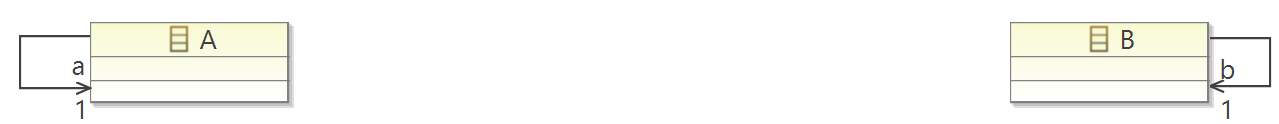
\includegraphics[width=0.9\textwidth]{MM2TinyIsomorph.png}
	\caption{Example (single class) MMa, MMb Metamodels.}
	\label{fig:MM2TinyIsomorph}
\end{figure}

The Class Diagrams in Figure~\ref{fig:MM2TinyIsomorph} show the `metamodel' for \verb|A| on the left and the corresponding `metamodel' for \verb|B| on the right.

\begin{figure}[h]
	\centering
	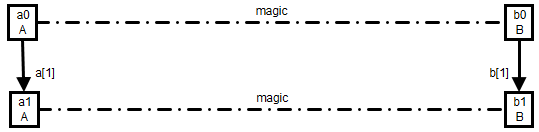
\includegraphics[width=0.9\textwidth]{InstancesTinyIsomorph.png}
	\caption{Example Instances.}
	\label{fig:InstancesTinyIsomorph}
\end{figure}

The Instance Diagrams in Figure~\ref{fig:InstancesTinyIsomorph} show our test input and output models. Two related \verb|A| instances on the left named \verb|a0| and \verb|a1|, and two similarly related instances of \verb|B| on the right named \verb|b0| and \verb|b1|. The dash-dotted lines indicate the magic performed by the transformation. For this simple, we can synthesize the super-optimal Java-like solution shown in Listing~\ref{lst:super-optimal}.

\begin{lstlisting}[label=lst:super-optimal,caption=Super-Optimal Example Conversion,captionpos=b]
// load a0, a1
B b0 = new B();
B b1 = new B();
b0.b = b1;
b1.b = b0;
// save b0, b1
\end{lstlisting}

Ignoring the load/save activities necessary to wrap the in-memory transformation as a practical application, we see two new statements and two assignments. Each new statement creates an output instance of the \verb|B| class. Each assignment populates the slot corresponding to the \verb|B::b| property with a resolved class reference. These necessary actions are performed without any additional control flow overhead.

The super-optimal solution demonstrates that the outputs can be created by interleaving new statements that create new instances, and assignment statements that assign the results of an OCL query to a slot of an instance.

The super-optimal solution, while correct, is of limited use since we need to generate a different super-optimal solution for each source model. We therefore prefer a less efficient solution that abstracts away from the run-time instances and slots to their compile-time classes and properties. This incurs some control flow overheads to accommodate a variety of input models as shown in Listing~\ref{lst:ideal-loop}.

\begin{lstlisting}[label=lst:ideal-loop,caption=Idealized Example Conversion Loop,captionpos=b]
// load allA
for (A anA : allA) {
    B aB = new B();
    aB.b = lookup(anA.a);
}
// save allB
\end{lstlisting}

The `for' loop over all source A elements is an obvious control overhead. The `lookup' operation is the distinguishing characteristic of model transformations; the ability of one part of a transformation to query conversions made by another part. 

\subsubsection{Java-like Example}

We will look at M2M solutions shortly. For now consider the Bad-Java-like solution shown in Listing~\ref{lst:bad-java-loop}.

\begin{lstlisting}[label=lst:bad-java-loop,caption=Bad-Java-like Example Conversion Loop,captionpos=b]
Map<A,B> a2b = new Map<A,B>();
// load a2b.keySet()
for (A anA : a2b.keySet()) {
    B aB = new B();
    a2b.put(anA, aB);
    aB.b = a2b.get(anA.a);
}
// save a2b.values()
\end{lstlisting}

A Map is used to correlate each input \verb|A| instance and its corresponding output \verb|B| instance, the keys of the Map are populated by the load. The \verb|lookup| is replaced by a \verb|put| of each created value followed by a \verb|get| of the referenced value.

Unfortunately, the Bad-Java-like Listing~\ref{lst:bad-java-loop} code only half-works, since perhaps half of the \verb|get| accesses may occur before the requisite \verb|put|. As is often the case with non-trivial conversions, it is necessary to perform the graph conversion in two passes. A first pass performs a tree traversal to establish the output equivalents and a second pass fills in the graph cross references. This is shown in Listing~\ref{lst:ok-java-loop}.

\begin{lstlisting}[label=lst:ok-java-loop,caption=Ok-Java-like Example Conversion 		Loop,captionpos=b]
Map<A,B> a2b = new Map<A,B>();
// load a2b.keySet()
for (A anA : a2b.keySet()) {    // tree-pass
    B aB = new B();
    a2b.put(anA, aB);
}
for (A anA : a2b.keySet()) {    // graph-pass
    B aB = a2b.get(anA);
    aB.b = a2b.get(anA.a);
}
// save a2b.values()
\end{lstlisting}

We can see that the memory overhead for this simple conversion requires a Map of input to output instances, and the control overhead requires two loops, and three Map accesses per element.

\subsubsection{Model-to-Model Transformation Solutions}

The \verb|lookup| capability is so fundamental to M2M, that all M2M languages provide a dedicated solution so that the Map is maintained internally.

In ATL \cite{Eclipse-ATL}, there is a `resolveTemp' built-in function to interrogate the Map. In Epsilon \cite{Eclipse-Epsilon} it's `equiv' and in QVTo it's `resolve'. The behaviour of these magic built-in functions is often poorly specified and programmers discover that they are using the Bad-Java-like solution the hard way. Sometimes the magic function works, sometimes it doesn't. The simplest way to get the transformation to work is to split the conversion into two passes, just like the Ok-Java-like solution; the first pass creates the output elements and populates the hidden Map. The second pass uses the magic built-in function after the hidden Map has been fully populated. This obviously requires the programmer to understand the hazard, to change the exposition to use two passes and to use some form of sequencing statement for the passes.

\subsubsection{QVTc Tracing}

\begin{figure}[h]
	\centering
	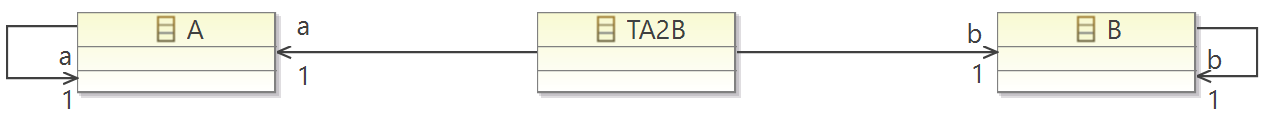
\includegraphics[width=0.9\textwidth]{MM3TinyIsomorph.png}
	\caption{Example (single class) MMa, Trace, MMb Metamodels.}
	\label{fig:MM3TinyIsomorph}
\end{figure}

In QVTc, the magic built-in function is reified by the trace class provided by the additional trace metamodel shown in the middle of Figure~\ref{fig:MM3TinyIsomorph}. 

\begin{figure}[h]
	\centering
	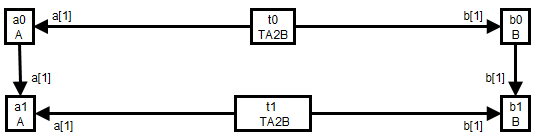
\includegraphics[width=0.9\textwidth]{TracedInstancesTinyIsomorph.png}
	\caption{Example Instances with Traces.}
	\label{fig:TracedInstancesTinyIsomorph}
\end{figure}

Figure~\ref{fig:TracedInstancesTinyIsomorph} shows how the magic mapping is replaced by a \verb|TA2B| instance with \verb|TA2B::a| and \verb|TA2B::b| slots locating the source and target instances with precisely \verb|[1]| multiplicity. In terms of memory usage, this is almost identical to the \verb|Map::Entry::key| and \verb|Map::Entry::value| fields that lie behind the Java Map implementation. However with a modeled magic function, the magic can be formalized by OCL navigation.

\begin{lstlisting}[label=lst:qvtc-loop,caption=Java-like Example Conversion Loops using the QVTc trace,captionpos=b,numbers=left]
// load allA
for (A anA : allA) {
    B aB = new B();
    TA2B a2b = new TA2B();
    a2b.a = anA;
    a2b.b = aB;
}
for (A anA : allA) {
    anA.TA2B.b = anA.a.TA2B.b;
}
// save allB
\end{lstlisting}

In Listing~\ref{lst:qvtc-loop} we show the use of OCL navigations, but continue to present it in a Java-like style to ease comparison and avoid the unnecessary confusion of a perhaps unfamiliar QVTc syntax.

This exploits one of the fundamental characteristics of OCL; all navigations may be traversed in either direction. Navigation directions without explicit names are given implicit names based on the target class names.

Thus the (forward) assignment of \verb|anA| to \verb|a2b.a|, at line 5, also makes the (reverse) assignment of \verb|a2b| to \verb|anA.TA2B| since \verb|A::TA2B| is the implicit opposite role name of \verb|TA2B::a|.

At line 9, the left hand side realizes the top traversal from \verb|a0| to \verb|t0| to \verb|b0| for \verb|lookup(anA)| as \verb|anA.TA2B.b|. Similarly on the right hand side, the bottom traversal \verb|a1| to \verb|t1| to \verb|b1| for \verb|lookup(anA.a)| is reified as \verb|anA.a.TA2B.b|.

\subsubsection{QVTr Tracing}

Behind the scenes, QVTr re-uses the QVTc trace. The QVTr concrete syntax makes the lookup available in a bidirectional fashion as shown in Figure~\ref{fig:QVTrTinyIsomorph}.

\begin{figure}[h]
	\centering
	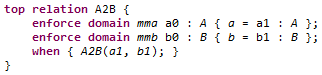
\includegraphics[width=0.6\textwidth]{QVTrTinyIsomorph.png}
	\caption{Example Mapping expressed as a QVTr Relation.}
	\label{fig:QVTrTinyIsomorph}
\end{figure}

Each \verb|domain|, one for the \verb|mma| and the other for the \verb|mmb| directions, defines the instance pattern shown at the left and right of Figure~\ref{fig:TracedInstancesTinyIsomorph}. The the \verb|a0|/\verb|b0| instance at the root of each pattern has a related \verb|a|/\verb|b| slot for an \verb|a1|/\verb|b1| instance.

The overall \verb|relation A2B| relates the \verb|a0|/\verb|b0| root of each pattern and is reified by the \verb|t0| trace shown at the top of Figure~\ref{fig:TracedInstancesTinyIsomorph}.

The additional \verb|when| clause requires that \verb|a1| and \verb|b1| are related by \verb|A2B(a1, b1)|. It is reified by the \verb|t1| trace shown at the bottom of Figure~\ref{fig:TracedInstancesTinyIsomorph}.

\subsection{Timing Hazards}

We have seen how in the Bad-Java-like solution the careless use of a Map can lead to malfunctions. This cuts right to the heart of the difference between a fully declarative program exposition and a traditional imperative / functional approach.

\subsubsection{Function Hazards}

A function \verb|F| has overt/explicit \verb|Inputs(F)| and \verb|Outputs(F)| which a programmer exploits to build a program whose execution can be analyzed by examining the call tree of the functions. However a function also has implicit inputs and outputs in the form of \verb|Gets(F)| and \verb|Puts(F)| for the memory accesses that occur within the function. We can ignore the further side-effects of the form \verb|News(F)| since in practice each new element is put somewhere for use by a subsequent get. It is sufficient to worry about ensuring that each element of \verb|Gets(F1)| is after the appropriate \verb|Puts(F2)|.

More formally, using:

\begin{itemize}
	\item \verb|Gets(F)| the read accesses of function \verb|F| / mapping \verb|M|
	\item \verb|Puts(F)| the write accesses of function \verb|F| / mapping \verb|M|
	\item \verb|Element(A)| the element referenced by an access \verb|A|
	\item \verb|SSA(A)| the `time' at which an access \verb|A| occurs
	\item \verb|SSA(E)| the `time' at which the assignment to \verb|E| occurs
	\item \verb|Ready(A)| whether an access \verb|A| occurs after its assignment
	\item \verb|Producers(E)| the inverse of \verb|Puts(F)|
	\item \verb|Consumers(E)| the inverse of \verb|Gets(F)|
\end{itemize}

We assume a Static Single Assignment formulation of the code. The `time' returned by the \verb|SSA(.)| function has sufficient granularity to enable its values to determine whether one `time' precedes another. The granularity might be wall-clock time on a single processor or pass numbers on a multi-processor.

The \verb|Ready| helper is therefore true when the `time' of the access follows the `time' of the assignment to the accessed element.

\begin{equation}
		Ready(A) = SSA(A) > SSA(Element(A))
\end{equation}

To avoid malfunction we require that all the gets of all functions are ready.

\begin{equation}
	\forall f \; : \; F \; \; \forall e : Gets(f) \; | \; Ready(e)
\end{equation}

Conventional languages provide no compile-time or run-time support for \verb|Ready| to ensure that the above is satisfied and so in a large program, the integrity of the design is entirely down to the diligence and skill of the programmer.

In more complicated programs there may be a selective manual reification of \verb|Ready| through the use of \verb|Map::containsKey| or just a \verb|null|/non-\verb|null| variable, However, it remains a manual programming responsibility to ensure that the selective \verb|Ready| disciplines are appropriate and respected.

Sadly, since programmers are human, timing violations occur resulting in program malfunctions and opportunities for exciting debugging sessions. Program maintenance is a particularly perilous undertaking since the maintaining programmers may fail to understand the informal disciplines that the original programmers used to keep problems under control.

\subsubsection{Mapping Hazards}

A mapping \verb|M| has a similar structuring using \verb|Inputs(M)| and \verb|Outputs(M)|, but for a fully declarative transformation there is no need for a manual guarantee that all \verb|Gets(M1)| follow the appropriate \verb|Puts(M2)|. Rather, every mapping invocation must check that each \verb|Gets(M1)| does follow the appropriate \verb|Puts(M2)|. If the check fails, the mapping invocation must be deferred for retry until the \verb|Puts(M2)| has occurred.

Run-time support for the \verb|Ready| helper is therefore necessary unless the tooling can discover an execution order that guarantees that everything is always ready in time. This is sometimes possible, but certainly not always. In practice the tooling can only look to finding a good execution order that minimizes the mappings/accesses for which the overheads of run-time \verb|Ready| support are necessary.

\subsection{Analysis}

Neither QVTr nor QVTc Abstract Syntax models are convenient for detailed analysis and so the Eclipse QVTd project has developed a lower level QVTs graphical representation and visualization that is suitable for analysis and schedule preparation. The visualization of the patterns underlying a mapping has many similarities to an instance diagram and consequently a Triple Graph Grammar \cite{TGG-Optimization}. However whereas a TGG is a manually developed program, QVTs diagrams are an auto-generated\footnote{The QVTs diagrams in this paper have auto-generated content but manually enhanced layout.} visualization of a declarative model transformation. 

\subsubsection{QVTs Tracing}

The QVTs visualization of our example is shown in Figure~\ref{fig:QVTsTinyIsomorph}. It is a purely declarative exposition of the state of each mapping invocation after the transformation completes. All relation semantics are reified by trace navigation.

\begin{figure}[h]
	\centering
	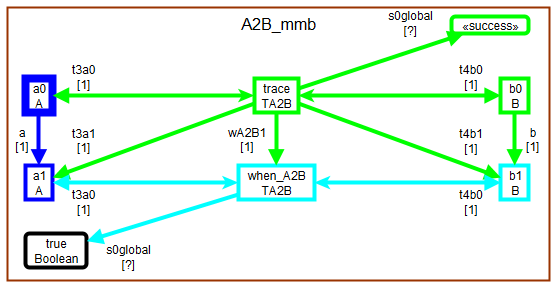
\includegraphics[width=0.8\textwidth]{QVTsTinyIsomorph.png}
	\caption{Example Mapping using QVTs.}
	\label{fig:QVTsTinyIsomorph}
\end{figure}

Contrasting Figure~\ref{fig:QVTsTinyIsomorph} with Figure~\ref{fig:TracedInstancesTinyIsomorph} the most obvious difference is the (auto-generated) coloring that animates the chosen directional execution towards \verb|mmb|.

\paragraph{Colors}
 
The colors indicate when the relevant elements are valid.
\begin{itemize}
	\item Black elements are all-time constants.
	\item Blue (loaded) elements are available after the input model is loaded.
	\item Green (produced) elements are created by successful execution of the mapping.
	\item Cyan (consumed) elements must be available before execution completes.
\end{itemize}

\paragraph{Invocation Status}

Two additional nodes at bottom left and top right reify the three-valued success, failure or not-ready status of an invocation using the \verb|true|, \verb|false| or\verb| null| values of the \verb|s0global| slot.

The upper central row shows the green creation of \verb|trace| and \verb|b0| instances corresponding to the incoming \verb|a0| instance. The \verb|t3a0| and \verb|t4b0| slots are populated so that the \verb|trace| instance captures the invocation. The special value \verb|«success»| is assigned to the status. If the invocation succeeds all green elements are created/assigned and the success status is \verb|true|. If the the invocation fails, only green trace elements are created/assigned and the status is \verb|false|.

The lower central row shows a topographically similar trace named \verb|when_A2B| from the \verb|a1| to \verb|b1| instance. The coloring is however cyan indicating that the elements are looked-up / re-used from elsewhere. The additional \verb|s0global| status constant at bottom left is a guard condition asserting that the referenced invocation completed and had a successful status.

The use of \verb|t3a1|, \verb|wA2B1| and \verb|t4b1| slots becomes apparent in Figure~\ref{fig:TinyIsomorphPartitions}.

\paragraph{Nodes and Shapes}

Each node identifies a pattern variable bound to a value or an instance by a successful match. The variable may have a name (above), and a type (below) that constrains possible matches.

Each rectangular node instantiates a metamodel \verb|Class|, such as \verb|A|, as a named-variable in the pattern.

Each rounded node instantiates a metamodel \verb|Datatype|, such as \verb|Boolean|, with a value in the pattern.

(Not shown in this example: Ellipses support \verb|Iteration| and \verb|Operation| calls.)

\paragraph{Edges and Arrows}

Each edge imposes further constraints on the permutations of model instances that can match the pattern. 

Each navigation edge instantiates a metamodel \verb|Property| as a constraint on the relationship between its two end nodes. At least one of the role names and multiplicities annotates the edge.

Whereas, in the Figure~\ref{fig:TracedInstancesTinyIsomorph} instance diagram, the arrows show UML navigability, the arrows in Figure~\ref{fig:QVTsTinyIsomorph} show whether the target is related to the source by something-to-zero/one multiplicity. Triangular arrow heads show the easily navigable paths declared in the UML metamodel. Chevron arrow heads show the potentially expensive paths provided by OCL opposites. No-arrow shows a path for which there may be multiple target instances per source instance/value.

(Not shown in this example: Argument edges support Iteration and Operation calls.)

\paragraph{Borders}

The navigation arrows identify nodes that can uniquely reached from other nodes. The closure of this relationship identifies a minimal set of nodes from which all nodes can be reached uniquely. We call this minimal set the head nodes and use a thicker border for them. In this example, a single node is sufficient, the \verb|a0| node. Therefore given an instance of \verb|A|, all other elements of a successfully matched pattern can be resolved by simple navigation. A practical schedule can loop over all \verb|A| instances and invoke the mapping binding the head to each instance in turn. It is not necessary to perform a mindless two-dimensional search of all possible matches for the two \verb|a0| and \verb|a1| pattern variables.

Occasionally two or more head nodes are required and two or more dimensional instance permutations are then necessary.

\subsubsection{Dependency Analysis}

The auto-generated QVTs decorations show the fruits of some simple multiplicity-based analysis, the multiplicity variously coming from the metamodel, transformation declarations and fundamental transformation semantics. The cyan and green coloring shows the analyzed consumer/producer behaviors.

Clearly green nodes are produced/created by some mapping and then consumed as cyan nodes by other mappings. These nodes are instances of model elements and may be passed as arguments to functions or mappings or stored in variables or collections.

Less obviously, green edges are produced/assigned by some mapping and consumed as cyan edges by other mappings. These edges are instances of model slots that typically lack a first class run-time representation. They cannot be passed around; rather the instance at one end can be passed together with an `instruction' as to which instance-slot to access. It is therefore tempting to simplify the edge analysis to re-use the source node analysis with a minor addition for the slot `instruction'.

However this simplification leads to a serious loss of precision and every loss of precision impairs the ability to discover an efficient schedule. It is often the case that in a relationship such as UML's \verb|Element::ownedElement|, one or both ends of the relationship is declared in the transformation to be of a more specific type than the \verb|Element| type declared in the metamodel. Without the extra precision we may find that any of perhaps ten possible producers of \verb|Element::ownedElement| can be consumed by any of perhaps ten possible consumers requiring a substantial 10*10 run-time permutation of the options. With the extra precision, we may find that each derived producer of \verb|Element::ownedElement| can be consumed by any of only one or two  possible consumers requiring no permutation at all or perhaps just a much reduced two or three way run-time permutation.

We therefore analyze each edge production as a triple \{\verb|production-source-type|, \verb|property|, \verb|production-target-type|\}. Subsequently determination of the producers for a consumption of a corresponding triple \{\verb|consumption-source-type|, \verb|property|, \verb|consumption-target-type|\} must consider all possible run-time matches rather than compile-time conformances. We can only reject a match when 
 \verb|production-type| does not conform to \verb|consumption-type| and vice-versa for either source and target types. This either way conformance is not very discriminating, but it is sufficient to distinguish consistent use of derived types.

\subsubsection{Operation Analysis}

A conventional operation execution is unable to fail and retry when a required slot is not ready. This conflicts with the retry-if-not-ready behavior of the declarative transformation run-time. We must find a solution that ensures that operations execute correctly. 

Banning operations is clearly unacceptable and re-implementing operation execution to support retries is very unattractive. We can however extend our dependency analysis to include deep analysis of operation invocations so that the invoking mapping checks the readiness on behalf of the called operation tree. This is tractable since we are dealing with OCL operations whose behavior is amenable to analysis and whose execution is side-effect free.

However a precise deep analysis of every polymorphic operation call tree is not always possible, so we must fall back on a slightly pessimistic analysis of every possible type usage and property access. Improved accuracy of polymorphic operation analysis is obtained by specializing the analysis to the actual types provided by the caller rather than the possible types supported by the operations.

\subsubsection{Endogenous Analysis}

An endogenous transformation uses the same types for input and output models. Consequently a class/property-based analysis will find that all the early `input' consumptions are in conflict with `output' productions. The dependency analysis concludes that just about everything depends on everything. This difficulty vanishes if each class/property is qualified by the domain direction that it contributes to.

\section{Cycles}\label{Cycles}

The naivest declarative execution repeatedly permutes all possible instances against all possible mappings until sufficient progress has been made to constitute completion.

In this paper we seek to discover as close as possible to a fully static schedule in which compile-time analyses determine an appropriate execution order for the mappings so that the run-time iterates over the instances, invokes only relevant mappings exactly once and completely avoids all overheads from maintaining the not-ready status of slots and premature mapping invocations. The auto-discovered static schedule does just what an omniscient manual programmer could have programmed. Of course for non-trivial mappings a real rather than omniscient programmer may accidentally invoke helpers redundantly and more seriously may fail to understand the required execution order and so may produce a buggy program.

%\subsection{Cycle Hazards}

%We have seen that the ideal schedule may comprise an explicit enumeration of new and assignment statements. Is this always possible? No. If 'your salary' is computed as \$100 more than 'my salary' and vice-versa, there is an insoluble contradiction. We can just hope that our compiler can detect the cyclic dependency and inconsistency before a naive run-time hangs searching all possible salaries for the solution. In some cases such as 'your salary is twice my salary' and 'my salary is \$100 more than your salary' a symbolic loop analysis may discover the disconcerting solution that your salary is -\$200. Analogously with proving that a program terminates, we need to recognise that some programs are fundamentally bad or at least too hard too analyze.

%In practice most cycle hazards are an artefact of using a compile-time analysis or an inappropriate solution exposition.

%A traditional program comprises a call tree of function calls. The programmer concentrates on the call tree and so the relationship between functions are required outputs is often rather distant. Ensuring that functions are called in appropriate order is a significant skill. The consequences of a poor order are at least inefficiency, more often malfunctions and major debugging headaches.

%A traditional model transformation is not that much better. The transformation language may be friendlier for model maintenance, but the need for an appropriate mapping call tree remains.

%A fully declarative transformation changes the situation completely. It is not necessary, perhaps not even possible, for the programmer to specify the call tree. Each mapping accurately specifies what to convert and how. The declarative transformation tool must discover the call tree, avoiding the hazards of bad sequencing and allowing the programmer to concentrate on what must be done without regard to how. In doing so the declarative programmer no longer needs to manually split the processing into passes, one for tree construction and another for cross-reference resolution as in our example. Rather the declarative can freely intermix usage of inherited attributes, computed top-down, with synthesized attributes, computed bottom-up. Such usage would normally require distinct passes. But no, the declarative tooling must sort it out.

%The basis for determining an efficient schedule is a complete global analysis to determine the producers and consumers of each class and/or property. Given such an analysis, it is 'simple' to place ensure that producers execute before their consumers.

%The fully declarative exposition of each mapping/relation/rule is much too big; it contains many assignments that depend on slots whose transitive dependencies create cycles. These are false cycles caused by the unnecessary requirement that a mapping executes atomically. Partitioning the mapping into smaller pieces just as the manual programmer would do can eliminate these cycles. We used to advocate \cite{Willink-EXE2016} a maximal partitioning so that each micro-mapping has at most one new or assignment statement breaks all the false cycles, but this creates a perhaps three-fold burden on the subsequent analyses that must deal with a much larger number of micro-mappings. Unless a later merge phase is introduced, these extra micro-mappings may incur run-time costs as well. We now advocate the extra effort of a just-right partitioning of as few mappings as possible into as few partitions as possible.

\subsection{Permutation Cycles}

Each naive permutation attempt results in a mapping invocation that may succeed and make a small quantum of progress towards the final result.

The simplest approach to reducing the number of fruitless permutations is to recognise that each mapping has a type signature that restricts the instances that can possibly conform.

A static compile-time analysis of the transformation can identify all the types that contribute to mapping signatures. At load-time, analysis of the input models can distribute the instances to type-specific bins so that during the subsequent execution only type-conformant instances are permuted. Inheritance complicates the picture slightly requiring either that some instances to be distributed to multiple bins or that multiple bins are used for some permutations.

For transformations with many mappings and for metamodels with many types, avoiding the irrelevant permutations may easily lead to an order of magnitude speed-up.

For non-trivial mappings the reduced search space dimensionality through accurate identification of the head node(s) is potentially the most significant optimization since it may give a speed up from cubic or quadratic to linear.

\subsubsection{Discriminants}

The type-based distribution of instances at load-time is easy for strongly-typed metamodels with access to the type via \verb|eClass()| in Ecore or \verb|xsi:type| in XMI.

Some applications have very weak metamodels with very few types making the simple type-based separation ineffective. However all is not lost since even weakly typed models often have a type discriminant such as a \verb|kind| string. Static analysis of the transformation can first identify candidate discriminants as the attributes that have constant assignments at the time of construction/production. Further examination of the attributes that have constant predicates at the time of consumption reveals which candidates usefully correlate a subset of all possible productions with a subset of all possible consumptions.

The use of discriminants is not limited to weakly-typed metamodels. A derived attribute such as container-is-null may usefully discriminate the root from a non-root element in a tree. This avoids permuting non-root elements to a root-only mapping and vice-versa. 

\subsubsection{Open Metamodels}

Many of the analyses and resulting optimisations in this paper rely on a complete metamodel analysis supporting a strong conclusion that type A either can or cannot conform to type B.

This analysis is unfortunately not safe if the load-time input instances may conform to an extension of the compile-time metamodel. For example, a transformation based on the UML metamodel may optimize to exploit the guarantee that a \verb|Class| instance cannot conform to the \verb|Package| type. Unfortunately, if the transformation is applied to a QVT model whose \verb|Transformation| class extends both \verb|Class| and \verb|Package|. A (derived) \verb|Class| instance may indeed be a (derived) \verb|Package| instance. The optimized transformation may well malfunction.

Examination of the QVT metamodel reveals that the problematic multiple inheritance is a quite disgraceful pragmatism that is easily removed, and indeed is removed in the Eclipse QVTd implementation. We therefore ignore the problems of open metamodels. If a user really requires dirty derived metamodels, the user should arrange to make these dirty metamodels visible at compile time.

\subsection{Not-Ready Cycles}

Whereas a traditional program malfunctions if some required input slot has not been computed, a declarative transformation fails but arranges to retry until the required slot has been computed. This imposes two undesirable run-time overheads. Firstly each failed mapping invocation must have an ability to be stored for a retry. And each required input slot must have a has-been-computed / not-ready status.

Each retry incurs additional overheads. These can be reduced by only retrying once the cause of the failure has been resolved. Since the failure is associated with a not-ready consumption of a slot, that slot can maintain a queue of mapping invocations waiting to retry once that slot is computed / produced. Correct correlation of production and consumption can be managed automatically by the declarative execution run-time. A corresponding manually maintained correlation in a traditional program is almost unthinkable.

Retrying only when there is a prospect of progress, reduces the number of attempts to typically two, rising only slightly for mappings that have multiple potentially not-ready input slots. This may give an order of magnitude performance improvement over mindless retries.

In the following sections we will examine how determination of a static schedule can guarantee that a mapping invocation only fails because of a predicate violation. The need to support retries is eliminated simplifying the execution dispatcher and eliminating per-slot not-ready status overheads.

\subsection{Compile-time Cycles}

The complete global analysis of all production/consumption dependencies between all mappings is, in the general case, a directed cyclic graph. Figure~\ref{fig:TinyIsomorphPrePartition} shows the dependency graph for our simple example.

\begin{figure}[h]
	\centering
	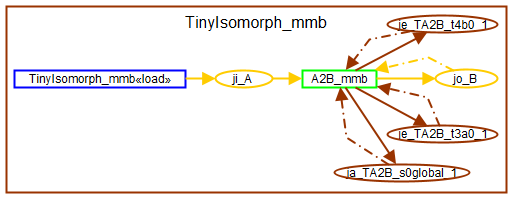
\includegraphics[width=0.8\textwidth]{TinyIsomorphPrePartition.png}
	\caption{Example Mapping Dependency Graph prior to Partitioning.}
	\label{fig:TinyIsomorphPrePartition}
\end{figure}

The blue rectangle shows the loader that passes loaded instances of \verb|A| to an orange input connection buffer named \verb|ji_A|. The instances are consumed by the green rectangle for the \verb|A2B| mapping in the \verb|mmb| direction. This mapping passes its produced \verb|B| instances to the output connection buffer named \verb|jo_B|. These output instances are also consumed.

The three brown ellipses support the equivalent production and consumption of edges such as the attribute buffer named  \verb|ja_TA2B.s0global_1|. Edge consumptions are hard to realize at run-time and so we would like to optimize them away.

The solid orange lines indicate paths along which instances flow and which can be realized at run-time. The dashed lines indicate consumption with a not-ready hazard. 

The four cycles for one node and three edges are not compatible with a simple tree-based schedule, we must therefore resolve. Our simple example contains only one mapping and is 100\% cyclic. For out example, we can skip over the considerations in the next section that identify cycles more generally.

\subsubsection{Cycle Encapsulation}

We can identify the cycles by computing from the green-producer/cyan-consumer analysis of  each mapping M as in Figure~\ref{fig:QVTsTinyIsomorph}.

\begin{itemize}
	\item \verb|pre(M)| - predecessors of M, the producers of the elements that M consumes
	\item \verb|suc(M)| - successors of M, the consumers of the elements that M produces.
	\item \verb|pre(M)*| - transitive closure of all predecessors of M
	\item \verb|suc(M)*| - transitive closure of all successors of M
	\item \verb|cyc(M)| - cycle involving M
\end{itemize}
	
We can observe that the mappings that appear in either \verb|pre(M)*| or \verb|suc(M)*| but not both are either transitive predecessors or successors of M and should be scheduled before or after M accordingly to ensure that the producer-consumer timing is unequivocably satisfied.

Conversely every mapping that appears in both \verb|pre(M)*| and \verb|suc(M)*| is part of the cycle involving M. The intersection of \verb|pre(M)*| and \verb|suc(M)*| identifies the \verb|cyc(M)| cycle members.

Mappings for which \verb|cyc(M)| is empty are acyclic; not part of cycles.

A static schedule can be produced for the acyclic mapping by allocating to a first pass all the mappings for which \verb|pre(M)*| is empty, then for subsequent passes allocating  the mappings for which \verb|pre(M)*| involves only mappings allocated to earlier passes. This provides a largely parallel schedule since concurrent execution on multiple processors is possible for each mapping in the same pass and each invocation of that mapping. Only passes need sequencing. All overheads in respect of not-ready slots or execution retries can be eliminated.

However in practice cycles do occur. The number of distinct non-empty values for \verb|cyc(M)| identifies the number of cycles.

If \verb|cyc(M1)| and \verb|cyc(M2)| have no common members, \verb|cyc(M1)| and \verb|cyc(M2)| are independent cycles.

If \verb|cyc(M1)| is a subset of \verb|cyc(M2)| then \verb|cyc(M1)| is a nested cycle within \verb|cyc(M2)|.

The third possibility of a non-subset overlap between \verb|cyc(M1)| and \verb|cyc(M2)| cannot arise since all cycle members are both predecessors and successors of each other.

Accommodating cycles within the static schedule proves to be remarkably easy. Each outer cycle has a distinct value of \verb|cyc(M)| that is not a subset of another cycle. The outer cycle can be wrapped in a cyclic-mapping \verb|CM| that is externally acyclic, and only internally cyclic. Since it is externally acyclic, it can be allocated to a pass in just the same was as the inherently acyclic mappings. We just need to ensure that invocations of the \verb|CM| are repeated until the internal cycle is satisfied and ensure that all consumed slots have run-time support for the not-ready that may result from execution of cycle elements in the `wrong' order.

Producing a static schedule for the members of the cycle is a nested problem. For scheduling we could resort to naive polling, but we can do better inspired by the principles of Structural Induction.

%The intersections for all M identify all the cycles. Each element of a cycle has the same intersections, so each distinct intersection identifies a distinct cycle. Nested cycles are of course possible; each element of the nested cycle is also part of the nesting cycle so the distinct intersection for a nested cycle is smaller than and fully contained by the distinct intersection of a nesting cycle.

%The cyclic directed graph can be converted to an acyclic directed graph by a Russian dolls approach. Starting with the smallest distinct intersection first, we wrap each cycle of mappings up inside a single nested cyclic mapping until no cycles remain. The resulting acyclic directed graph can be scheduled more easily, just taking care to repeat each nested cyclic mapping for as long as necessary. 

For each mapping M in the cycle we can classify its dependencies as
\begin{itemize}
	\item \verb|ext(M)| the predecessors of M outside the cycle
	\item \verb|int(M)| the predecessors of M inside the cycle
\end{itemize}

A mapping with an empty ext(M) is dependent on some other cycle member and so is a `recursive' case. Conversely a mapping with a non-empty ext(M) may be able to execute directly and so is a `basic' case.

The conventional `base' case is an acyclic preamble. It would have an empty \verb|ext(M)| and \verb|int(M)|. It is not part of the cycle.

The `basic' cases have a higher probability of successful execution. Their execution attempts can therefore be scheduled first and their dependencies eliminated to allow the remaining `recursive' cases to be scheduled in acyclic dependency order. An overall surrounding loop repeats for as long as necessary. Extraction of the `basic' cases improves the initial hit rate and the ordering within the loop avoids premature scheduling of mappings that have no hope of successful execution.

In practice many loops are trivially small or shallow but polymorphically wide limiting the effectiveness of these optimizations.

\subsubsection{Partitioning}\label{Partitioning}

A typical mapping involves multiple productions and consumptions and may exploit the declarative freedom to intermix inherited attributes, computed top-down, and synthesized attributes, computed bottom-up \cite{Aho+Sethi+Ullman/86/Compilers}. This leads to many `false' cycles, cycles that are an artefact of the convenient declarative exposition rather than a necessary characteristic of the problem. At its simplest a mapping has production that after transitive consumption and production by other members of the cycle is consumed by the original mapping. Since the consumption occurs in the same mapping as the production, the successful consumption is a guard upon the production, but the consumption will fail with a not-ready until the production propagates. Deadlock and since this is exactly what the declarative programmer has specified, it is what we must do. To break the deadlock, we must execute at least one of the productions before their predicating consumptions without changing the overall result.

Fortunately not all consumptions and not all productions are equivalent. Figure~\ref{fig:QVTsTinyIsomorph} is drawn with three columns, the input/left, the trace/middle and the output/right column. No productions occur in the input column. The required externally observable productions occur in the output column. Hidden internal productions occur in the middle column.

In the absence of a complicated facility to roll-back misguided output element creations, we must only perform correct output element creations. However the internal trace provides some flexibility which we exploit by providing the \verb|s0global| status, this is \verb|true| if the trace is good, and \verb|false| if the trace fails or is misguided.

Consumptions of the input model elements typically check for some type/existence constraint. These do not present cyclic problems since the input is available.

Consumptions of the trace model elements typically check that some other execution has happened. This may lead to a cyvle that needs speculation.

Consumptions of output model elements may take two forms, corollaries or post-conditions.
A corollary occurs as in Figure~\ref{fig:QVTsTinyIsomorph} when a consumed trace/output object pair is topologcally identical to the trace/output pair in the corresponding producing mapping. If the producer creates the trace and assigns a success, the eventual production of the output is guaranteed to occur. It is therefore sufficient for the consumer to check the consuming trace and its status to determine whther the consuming mapping can be declared successful. The consumed output does not need to exist when success is declared.
 

Traditionally such usage would require manual separation into distinct passes.

Since the `false' cycles arise from `too-many' productions or consumptions per-mapping, we can solve it by emulating the manual partitioning by replacing each too-big mapping by multiple partitions.

The

%Partitioning incurs overheads through introduction of extra partitions to schedule so we want to minimize this. We do this in three stages:
%\begin{itemize}
%	\item a first cycle analysis identifies cyclic mappings
%	\item cyclic mappings are partitioned
%	\item a second cycle analysis identifies rather fewer cyclic partitions
%\end{itemize}

\paragraph{Production Partitioning}

Most productions contribute solely to the output from the mapping and so a partitioning to place each production in a distinct partition is possible and in accord with our advocation in \cite{Willink-EXE2016} to create as many `atomic' micro-mappings as possible. The cost of too-many micro-mappings was mitigated by a merge of similar micro-mappings as part of the overall partitioning and scheduling. 

The combined behavior of the partitions must  be identical to the original mapping and so each partition must repeat the predicate checks to ensure that each fails identically. With the same predicates, many of the per-production partitions have identical behavior that can be merged. It is however more effective to avoid over-partitioning. In practice the productions fall into four categories

\begin{itemize}
	\item \verb|«ctor»| creation of the unique trace element for the mapping invocation
	\item \verb|«init»| creation of the input-side trace edges
	\item \verb|«rest»| creation of the output-side nodes and trace edges
	\item \verb|«xtra»| creation of the output-side edges	
\end{itemize} 

\paragraph{Comsumption Partitioning}

Production partitioning is fairly straightforward since a production cannot fail. In contrast a consumption can, either temporarily until a slot is ready, or finally if the consumed object is of an unsatisfactory type or value.

\paragraph{Selective Partitioning}

The cycle analysis applied to the mappings identifies which mappings can be scheduled acyclicly and which need to form part of a cycle. There is no point partitioning acyclic mappings, so we concentrate our efforts on the typically small and sometimes zero number of cyclic mappings. Once we have partitioned the cyclic mappings, we can repeat the cycle analysis and often discover that many of the cycles were `false' cycles and so the partitions can be statically scheduled. Only the `true' cycles need incur the extra run-time overheads.

\paragraph{Partition Content Selection}

Safe, guaranteed to be ready/valid, consumptions provide no benefit when partitioned. Unsafe, possibly not-ready/not-valid consumptions cannot be partitioned since a partial mapping must not succeed when the overall mapping would have failed. Partitioning is therefore restricted to productions. 

In \cite{Willink-EXE2016}, we advocated a maximal partitioning into micro-mappings so that each micro-mapping has at most one green creation or assignment element to break many of the `false' cycles, but this imposes a perhaps three-fold burden on the subsequent analyses that must deal with a much larger number of micro-mappings. Unless a later merge phase is introduced, these extra micro-mappings may incur run-time costs as well. We now advocate the extra effort of a just-right partitioning of as few mappings as possible into as few partitions as possible; green elements with shared consumptions can remain together, but those with distinct dependencies can be separated. This typically results in some or all of:
\begin{itemize}
	\item a \verb|«ctor»| partition to create the trace linked to input roots
	\item a \verb|«init»| partition to check predicates and assign green trace-to-input edges
	\item a \verb|«loop»| partition to speculate and create green trace-to-output edges
	\item a \verb|«rest»| partition to assign green output-to-output edges
	\item a \verb|«xtra»| partition to assign green output-dependent edges 
\end{itemize} 

However partitioning productions is insufficient to break all the `false' cycles. In Figure~\ref{fig:QVTsTinyIsomorph} we see a very common green production pattern whereby the mapping creates a \verb|trace| trace element an output element \verb|b0| with a linking trace element \verb|trace.t4b0| with a status \verb|trace.s0global| that will be true whenever \verb|trace.t4b0| and \verb|b0| are valid. A similar cyan consumption pattern for \verb|when_A2B|, \verb|b1|, \verb|when_A2B.t4b0| is guarded by a requirement that the status \verb|when_A2B.s0global| is \verb|true|. It is therefore sufficient to check that \verb|when_A2B| exists and that \verb|when_A2B.s0global| is \verb|true| to guarantee that \verb|when_A2B.t4b0| and \verb|b1| are available. We therefore call \verb|b0| a corollary of \verb|A2B|; we can omit \verb|when_A2B.t4b0| and \verb|b1| from partitions provided \verb|when_A2B.s0global| is checked for \verb|true|. Elimination of dependencies on corollaries significantly reduces the number of output dependencies.

\begin{figure}[h]
	\centering
	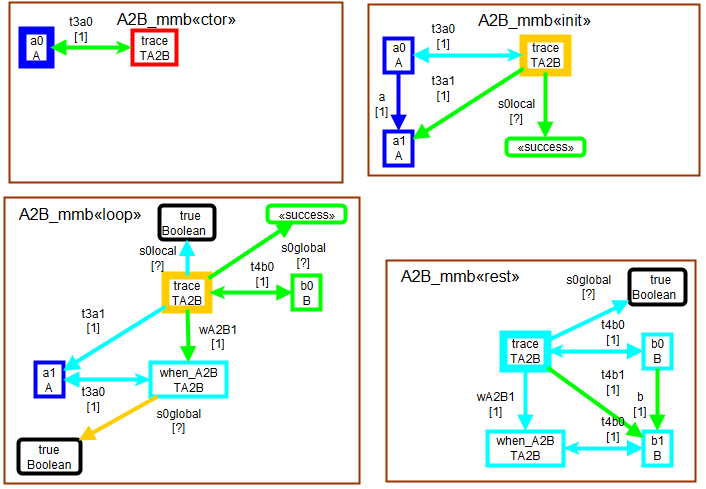
\includegraphics[width=1.0\textwidth]{TinyIsomorphPartitions.png}
	\caption{Partitions for Example Mapping.}
	\label{fig:TinyIsomorphPartitions}
\end{figure}

Figure~\ref{fig:TinyIsomorphPartitions} shows the content of the four partitions, with two new colors. Red for an not yet initialized trace and orange for elements participating in a speculation. The additional \verb|s0local| status prevents the \verb|«loop»| satring before \verb|«init»| has finished.

Figure~\ref{fig:TinyIsomorphPostPartition} shows the Dependency Graph for our simple example after it has been partitioned.

\begin{figure}[h]
	\centering
	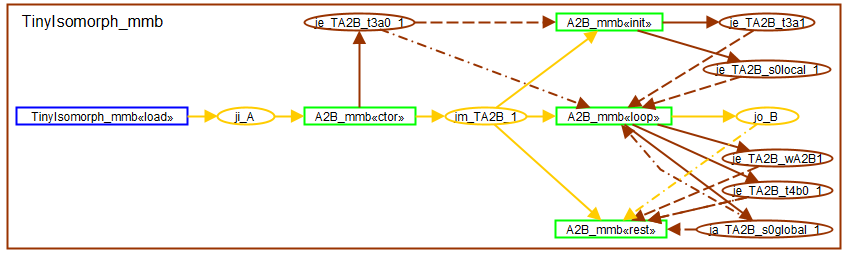
\includegraphics[width=1.0\textwidth]{TinyIsomorphPostPartition.png}
	\caption{Example Mapping Dependency Graph after Partitioning.}
	\label{fig:TinyIsomorphPostPartition}
\end{figure}

There are now four green partitions with the \verb|«ctor»| partition consuming the \verb|A| input and passing the \verb|TA2B| traces via the \verb|jm_TA2B_1| connection to the other three. All the cycles except that involving the \verb|s0global| status have been broken.

We can now allocate the partitions to passes. Figure~\ref{fig:TinyIsomorphFinal} shows the Dependency Graph after partitions and connections have been labeled with pass-numbers.  and after removal of all edges whose productions are guaranteed to occur in an earlier pass than all its consumptions.  

\begin{figure}[h]
	\centering
	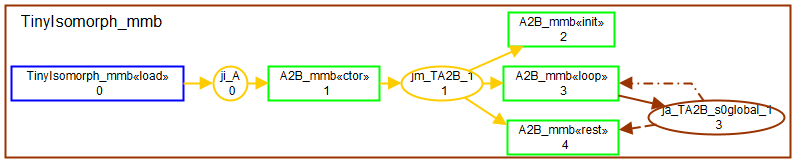
\includegraphics[width=1.0\textwidth]{TinyIsomorphFinal.png}
	\caption{Example Mapping Dependency Graph with Schedule Passes.}
	\label{fig:TinyIsomorphFinal}
\end{figure}

We are left with five passes for the overall \verb|«load»|, and the \verb|«ctor»|, \verb|«init»|, \verb|«loop»|, \verb|«rest»| partitions of the one mapping. Only one slot requires the ready/not-ready status to be maintained at run-time.

(Folding the «ctor» partition into its caller is future work.)

(Folding the «loop» partition into the «init» partition is future work justified in Section~\ref{Infallible Mappings}.)

\subsection{Run-time Cycles}

Where our compile-time analysis fails to eliminate a potential cycle, we need the run-time to resolve it.

It is easy to assume that even a naive scheduler that keeps trying all possible permutations of objects and mappings will eventually make progress and produce the required output. This is true of most practical transformations, but not necessarily so because each mapping may have a guard that inhibits execution unless some conditions are satisfied.

\subsubsection{Speculation}

Consider the very simple game: I'll show you mine, if you show me yours.

There are two stable outcomes; we both show or we both hide. There are also two outcomes where one of us cheats. The possibility of cheating can be eliminated by introducing a mediator. The result can be made deterministic if the mediator directs the play with a bias towards maximum disclosure.

A similar situation may arise in a model transformation. Which of multiple do-nothing or multiple do-something is appropriate? `the whole truth' principle provides the solution: do-nothing omits a legitimate action, it is not a whole-truth and so we can require maximum transformation. For many cases, this maximum disclosure/execution renders the mediator redundant, since the mediator always directs the players to show.

Let us elaborate our two person game to a multi-person ring: I'll show to the right if the left shows to me. The need for a mediator is now more important, but again redundant if the mediator always directs all players to proceed.

If we differently elaborate our game with a player who declines to gamble on the sabbath, the outcome of the game is still deterministic, but we need our mediator to determine whether everyone is prepared to play, before directing play for the consistent outcome. The analogous situation in a model transformation may arise through model or transformation polymorphism; some model elements may behave differently to others.

At run-time the mapping invocation inter-dependencies may form many graphs. The run-time therefore blocks each invocation that needs a speculation verdict from the mediator until all such invocations have been blocked. The mediator can then perform an AND function to determine whether all participants are prepared to play and release the blocked invocations with the appropriate successful/failed speculation.

Now consider a different elaboration of our game with rogue players whose behavior to the right is the opposite of that from the left. With an odd number of rogue players, we have a contradiction around the loop. With an even number of rogue players, there may be multiple outcomes with the maximum disclosure dependent on the relative positioning of the rogue players. There may be no unique maximum solution. This is a bad game. Likewise we must be prepared for the possibility that a transformation may be bad. The rogue player has introduced a NOT to complicate our logic, so that rather than checking the obviously unique hypothesis that all invocations can be successful with an AND gate, we need to search for a unique pattern of successful and failing invocations to satisfy the arbitrary logic that NOT and AND facilitate. Even for our simple example we can see that it is bad. Anything more complicated may require an impractical computation to determine the not-necessarily unique result. It seems better to declare these as bad at the outset.

Consider a resilient persistence transformation that has two alternatives, either to save using a DataBase or to use XML serialization; either may fail. The author may seek to minimize wasted execution by specifying saveInDB XOR saveInXML, but XOR hides an underlying NOT. What is the transformation supposed to do if both saveInDB and saveInXML are successful? It is a bad transformation and should be rejected as such and at the earliest possible opportunity.

\subsubsection{Special Cycles}

We have identified that acyclic run-time dependencies can be handled without incurring the overheads of speculation support. It is therefore beneficial to identify situations were the run-time dependencies can be guaranteed to be acyclic.

\paragraph{Composite Relationships}

UML (and Ecore) imposes a constraint that no instance can have more than one container. Consequently any cycle whose elements are inter-dependent solely because of a container/containment relationship is guaranteed to be acyclic; speculation support is not needed.

\paragraph{Infallible Mappings}\label{Infallible Mappings}

Some mappings and metamodels are so simple that once constructed with a conformant head node there is no other mechanism for the mapping to fail. The `mediator' is guaranteed to direct a speculation success. This is the case with our running example. The redundant speculation should be detected, The test for the \verb|s0status| is redundant and so distinct \verb|«loop»| and \verb|«init»| partitions are unnecessary. We should have just \verb|«init»| and \verb|«rest»| partitions similar to the manual solution.

\subsubsection{Overriding Mappings}

The QVT specification is somewhat vague as to the precise semantics of mapping overrides. It is therefore left to the Eclipse QVTd project to apply `the whole truth' principle to specify that as many mapping invocations as possible should be attempted, and the `nothing but the truth' principle to specify that no mapping invocation should be attempted if an overriding mapping invocation is successful. This amounts to a NOT predicate on each potential override which is not consistent for no-NOTs in a run-time speculation. Fortunately the primary speculation is on the polymorphic invocation which is positive. The  individual overrides do not comeinto play until the polymorph has been speculated.

%\subsubsection{Termination}

%With a surrounding loop that loops for as long as necessary, we need to establish that the loop makes progress and terminates. Termination is easy, there is a finite number of model elements, but progress?

\section{Related Work}\label{Related Work}

Existing model to model transformation tools such as ATL, Eclipse QVTo, Epsilon and Henshin \cite{Eclipse-Henshin} do very little if any static analysis or optimization. This work on static analysis and optimization of declarative schedules and metamodels using micromappings and connections appears to be almost completely novel. 

In the Triple Graph world, a catalogue of optimizations has been proposed \cite{TGG-Optimization}; domain driven applicability, caching/indexing, static analysis, incremental execution. Many of these come for free in the current work.

The explicit middle model imposed by QVTc traceability reifies a trace object so that to-one navigation paths between source and target can be very cheap and optimized to avoid more expensive paths.
% The use of the 'wrong' domain is not expensive.
The trace object is an inherent cache of related information. Indexing is an OCL-level further work optimization. 
%Local and global analyses for the Micromapping Model of Computation have been described in the preceding sections.

%Incremental execution has not been discussed in this paper. The Connections shown in Figure~\ref{fig:ExecutionContext} are well suited to incremental and concurrent execution.

Although not discussed in this paper, the utility of Connections shown as ellipses in Figures~\ref{fig:TinyIsomorphPrePartition}, ~\ref{fig:TinyIsomorphPostPartition}, ~\ref{fig:TinyIsomorphFinal} for incremental execution is demonstrated by the Eclipse implementation.

Detailed comparison of the approaches is quite hard, since it is very easy to provide a really bad reference implementation against which almost any sensible implementation will appear fantastic. Erly results demonstarting the performance were presented in \cite{Willink-EXE2016}.

This work diverged from an early Epsilon prototype to exploit the very strong limitations imposed by metamodels and declarative mappings. It therefore uses heuristics to produce a useful schedule relatively quickly, rather than exploring a large number of alternative schedules in an infeasible time \cite{Horacio-planning}.

%\section{Status and Further Work}\label{Status}

%The approach has evolved from an early Epsilon prototype through rewrites in Java to produce a usable tool. The next rewrite should use QVTr/UMLX as the programming language to further demonstrate their utility and to achieve the benefits of incremental code generation to enhance compilation times.

\section{Conclusion}\label{Conclusion}

We have demonstrated how detailed analysis of declarative transformations and metamodels can avoid the potentially horrendous performance of a naive execution.

\begin{itemize}
	\item Type analysis avoids needless permutations.
	\item Head node identification minimizes search match dimensionality.
	\item Producer/consumer analysis guarantees a correctly sequenced execution, enables cycle detection and minimizes not-ready cycling.
	\item Partitioning breaks many compile-time cycles.
	\item Efficient run-time support reduces not-ready support and supports the speculation necessary to handle the residual run-time cycles.
\end{itemize}

%We have described optimizations that support derivation of an efficient schedule for  QVTc, QVTr and UMLX.

Results of the first optimized code generated implementation show that declarative transformations can approach the performance of manually coded transformations \cite{Willink-EXE2016}.  

\backmatter

\bibliographystyle{alphaurl}
\bibliography{CyclicScheduling}

\abouttheauthors

\begin{acknowledgments}
Many thanks to Horacio Hoyos Rodriguez for the graphical perspective and Epsilon prototype and to all Dimitris Kolovos' team for insightful discussions.
\end{acknowledgments}

\end{document}


